% Metódy inžinierskej práce
\documentclass[10pt,twoside,slovak,a4paper, colorinlistoftodos]{article}
\usepackage{todonotes}
\usepackage[slovak]{babel}
\usepackage[IL2]{fontenc} 
\usepackage[utf8]{inputenc}
\usepackage{graphicx}
\usepackage{url} % príkaz \url na formátovanie URL
\usepackage{hyperref} % odkazy v texte budú aktívne (pri niektorých triedach dokumentov spôsobuje posun textu)
\usepackage{times}
\usepackage{cite}
\usepackage[demo]{graphicx}
\usepackage{subfig}

\pagestyle{headings}

\title{Personalizovaný hudobný odporúčací systém založený na CNN\thanks{Semestrálny projekt v predmete Metódy inžinierskej práce, ak. rok 2024/25, vedenie: PaedDr. Pavol Baťalík}} 

\author{Peter Uhrin\\[2pt]
	{\small Slovenská technická univerzita v Bratislave}\\
	{\small Fakulta informatiky a informačných technológií}\\
	{\small {xuhrinp@stuba.sk}}}

\date{\small 30. september 2024} 


\begin{document}


\maketitle

\begin{abstract}

Písať ku danej téme ma usmernil článok "Music content personalized recommendation system based on a convolutional neural network" 
https://link.springer.com/article/10.1007/s00500-023-09457-2

Dynamický rast A.I. v posledných rokoch a jeho implementácia preformovala hudobný priemysel na biliónový biznis. Čistá hodnota streamovacích platforiem je sumarizovane 19,4 bilióna USD. Využitie konvolučných neurónových sietí ovplyvnilo nielen distribúciu prostredníctvom na mieru generovaných playlistov, ale aj produkciu a vývoj vďaka rozsiahlemu dosahu, ktorý umožňuje presadiť sa širokej škále umelcov, ktorých rozmach spojený s vysokou diverzitou dotvára potrebu kvalitnej dátovej analýzy pre algoritmy pracujúce na hĺbkovom učení, ktoré pokiaľ majú dostatok informácií o interakciách rôznych používateľov na danej stránke tak dokážu poskytnúť relevantné odporúčania, čím zvyšujú kvalitu služby a udržiavajú konzumenta, teda zvyšujú priemerný strávený čas, čo vedie k zvyšovaniu tržieb skrz predaj reklamy a prémiových doplnkov. V počiatkoch sa využívaná umelá inteligencia, resp. nástroje hĺbkového učenia museli spoliehať najmä na 'kolaboratívne filtrovacie techniky' ktoré boli základom vtedajších verzií odporúčacích systémov. Tieto sa postupom času ukázali ako nedostatočné pretože nedokázali vytvoriť trefné návrhy pre nových používateľov, ani dostať do ich playlistov pomerne neznáme skladby. Pracovali najmä podľa interakcií a kompletne ignorovali vnútorné charakteristiky jednotlivých nahrávok. Dnešné systémy analyzujú a vyhodnocujú každý aspekt audio súborov, ako napríklad opakované vzory, text či dokonca 'emočné tóny' merajúce úroveň výšok tónov hlasu. Vďaka týmto vysoko sofistikovaným technikám dnes dokonca vzniká paradox voľby pre neobmedzený prístup k hudobným knižniciam všetkých žánrov a ér, kvôli čomu sa ľuďom ťažšie vyberá hudba presne podľa ich vkusu.

\end{abstract}



\section{Úvod}

\section{Úvod}

\begin{figure}
\centering
\begin{minipage}{.5\textwidth}
  \centering
  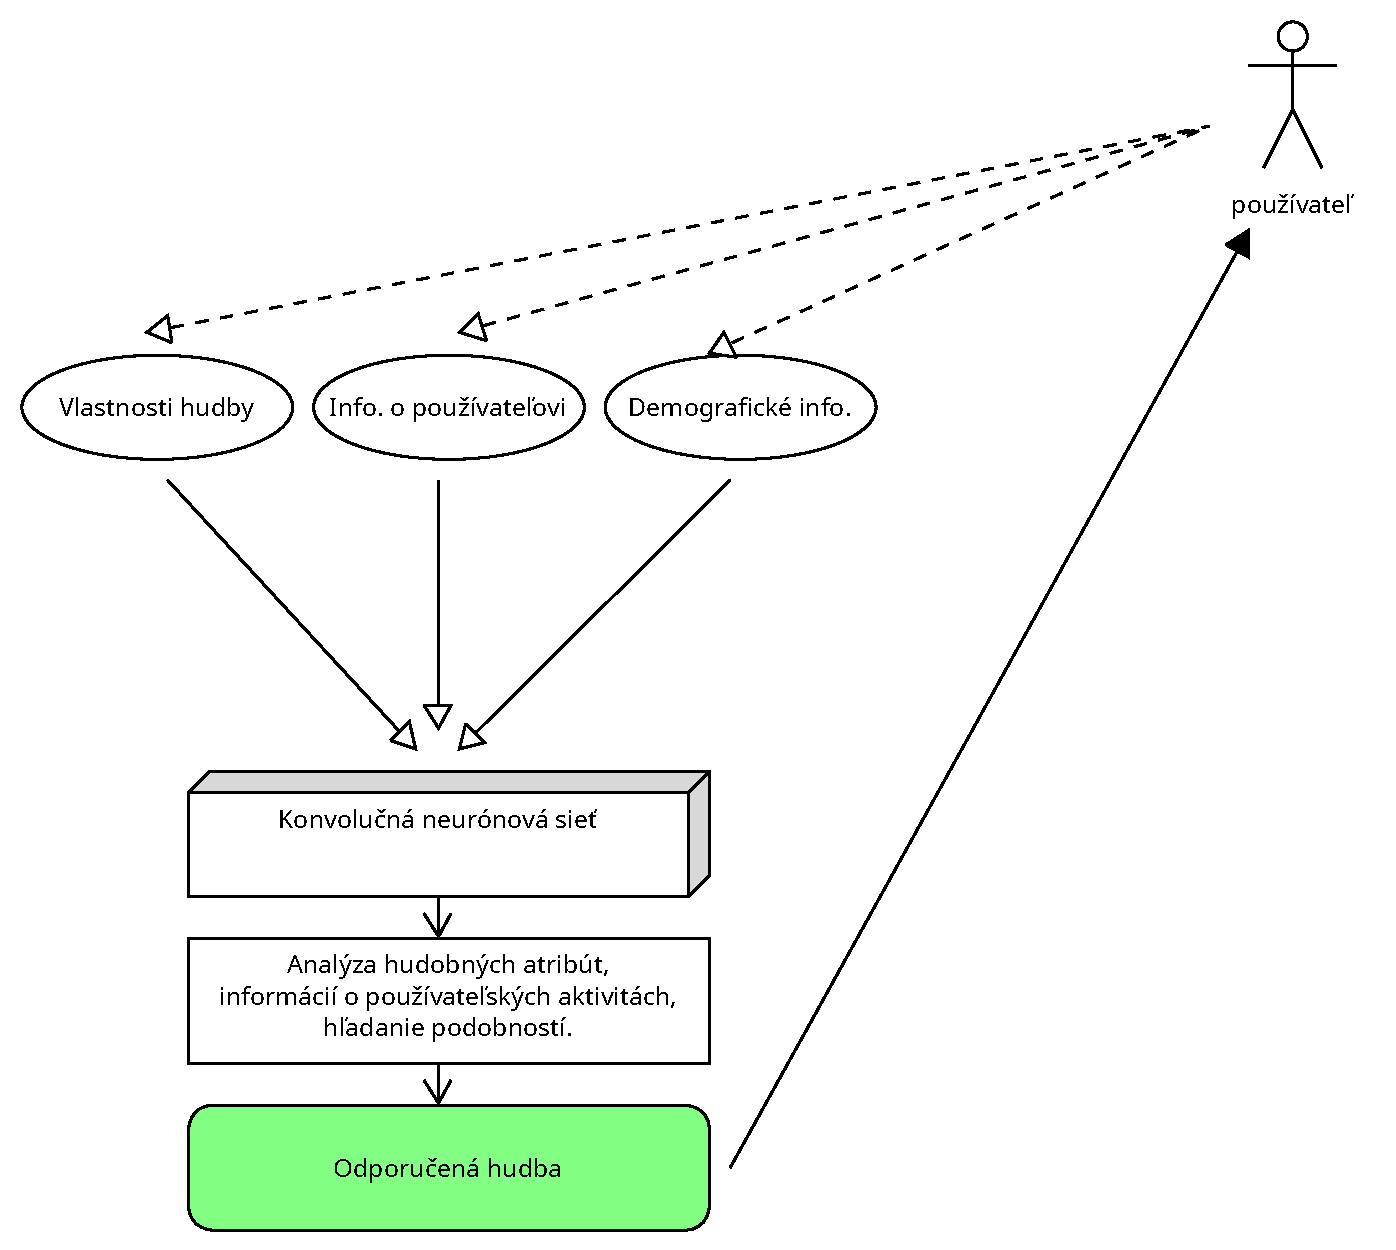
\includegraphics[width=.4\linewidth]{graf1.pdf}
  \captionof{figure}{A figure}
  \label{fig:test1}
\end{minipage}%
\begin{minipage}{.5\textwidth}
  \centering
  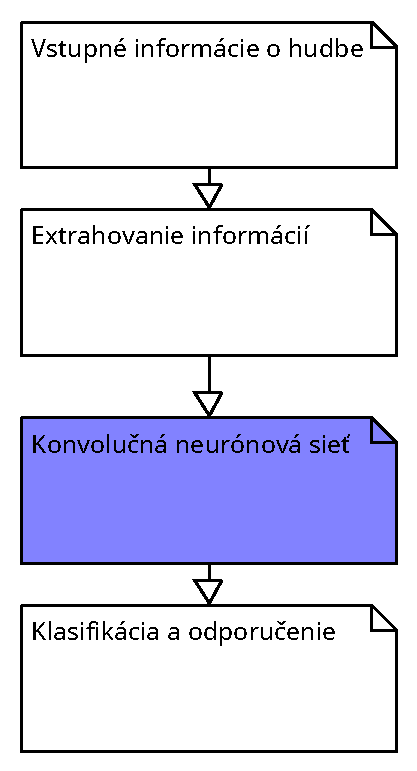
\includegraphics[width=.4\linewidth]{graf2.pdf}
  \captionof{figure}{Another figure}
  \label{fig:test2}
\end{minipage}
\end{figure}

Motivujte čitateľa a vysvetlite, o čom píšete. Úvod sa väčšinou nedelí na časti.

Uveďte explicitne štruktúru článku. Tu je nejaký príklad.
Základný problém, ktorý bol naznačený v úvode, je podrobnejšie vysvetlený v časti~\ref{nejaka}.
Dôležité súvislosti sú uvedené v častiach~\ref{dolezita} a~\ref{dolezitejsia}.
Záverečné poznámky prináša časť~\ref{zaver}.



\section{Personalizovaný odporúčací systém na hudobných streamovacích platformách} \label{1}
\subsection{Konvolučná neurónová sieť} \label{1:1}
\subsection{Algoritmy založené na hĺbkovom učení} \label{1:2}
\subsection{Algoritmy založené na obsahu} \label{1:3}
\subsection{Algoritmy založené na výpočte zhody} \label{1:4}
\subsection{Alogirtmy založené na CNN} \label{1:1}

Z obr.~\ref{f:rozhod} je všetko jasné. 

\begin{figure*}[tbh]
\centering
%\includegraphics[scale=1.0]{diagram.pdf}
Aj text môže byť prezentovaný ako obrázok. Stane sa z neho označný plávajúci objekt. Po vytvorení diagramu zrušte znak \texttt{\%} pred príkazom \verb|\includegraphics| označte tento riadok ako komentár (tiež pomocou znaku \texttt{\%}).
\caption{Rozhodujúci argument.}
\label{f:rozhod}
\end{figure*}



\section{Iná časť} \label{ina}

Základným problémom je teda\ldots{} Najprv sa pozrieme na nejaké vysvetlenie (časť~\ref{ina:nejake}), a potom na ešte nejaké (časť~\ref{ina:nejake}).\footnote{Niekedy môžete potrebovať aj poznámku pod čiarou.}

Môže sa zdať, že problém vlastne nejestvuje\cite{Coplien:MPD}, ale bolo dokázané, že to tak nie je~\cite{Czarnecki:Staged, Czarnecki:Progress}. Napriek tomu, aj dnes na webe narazíme na všelijaké pochybné názory\cite{PLP-Framework}. Dôležité veci možno \emph{zdôrazniť kurzívou}.


\subsection{Nejaké vysvetlenie} \label{ina:nejake}

Niekedy treba uviesť zoznam:

\begin{itemize}
\item jedna vec
\item druhá vec
	\begin{itemize}
	\item x
	\item y
	\end{itemize}
\end{itemize}

Ten istý zoznam, len číslovaný:

\begin{enumerate}
\item jedna vec
\item druhá vec
	\begin{enumerate}
	\item x
	\item y
	\end{enumerate}
\end{enumerate}


\subsection{Ešte nejaké vysvetlenie} \label{ina:este}

\paragraph{Veľmi dôležitá poznámka.}
Niekedy je potrebné nadpisom označiť odsek. Text pokračuje hneď za nadpisom.



\section{Dôležitá časť} \label{dolezita}




\section{Ešte dôležitejšia časť} \label{dolezitejsia}




\section{Záver} \label{zaver} % prípadne iný variant názvu



\section{Zaver 2}


%\acknowledgement{Ak niekomu chcete poďakovať\ldots}


\bibliography{lit}
\bibliographystyle{alpha} 
\end{document}



%\acknowledgement{Ak niekomu chcete poďakovať\ldots}


% týmto sa generuje zoznam literatúry z obsahu súboru literatura.bib podľa toho, na čo sa v článku odkazujete
\bibliography{literatura}
\bibliographystyle{plain} % prípadne alpha, abbrv alebo hociktorý iný
\end{document}
